\subsection{Q10.14 data 09202021 10082021 10312021 11092021 grouped by scenario \& PGM}

\begin{comment}
                             EFPR        EO      EFNR     n    pvalue
(frauth, Advantaged)     0.445455  0.554545  0.454545  55.0  0.421700
(frauth, Disadvantaged)  0.404762  0.595238  0.476190  21.0  0.353111
(icu, Advantaged)        0.567568  0.432432  0.567568  37.0  0.080939
(icu, Disadvantaged)     0.351852  0.648148  0.555556  27.0  0.151616
(rent, Advantaged)       0.367647  0.632353  0.441176  34.0  0.107199
(rent, Disadvantaged)    0.407895  0.592105  0.421053  38.0  0.410782
\end{comment}

\begin{table}[h]
    \centering
    \begin{tabular}{|c|c|c|c|c|c|c|}
        \hline
        scenario & PGM & EFPR & EO & EFNR & n & p-value\\
        \hline
        frauth & Advantaged & 0.445 & \textbf{0.555} & 0.455 & 55.0 & 0.422\\
		frauth & Disadvantaged & 0.405 & \textbf{0.595} & 0.476 & 21.0 & 0.353\\
		icu & Advantaged & \textbf{0.568} & 0.432 & \textbf{0.568} & 37.0 & 0.081\\
		icu & Disadvantaged & 0.352 & \textbf{0.648} & \textbf{0.556} & 27.0 & 0.152\\
		rent & Advantaged & 0.368 & \textbf{0.632} & 0.441 & 34.0 & 0.107\\
		rent & Disadvantaged & 0.408 & \textbf{0.592} & 0.421 & 38.0 & 0.411\\
		
        \hline
    \end{tabular}
    \caption{Grouped by scenario PGM}
    \label{tab:my_label}
\end{table}
\begin{figure}[h]
    \centering
    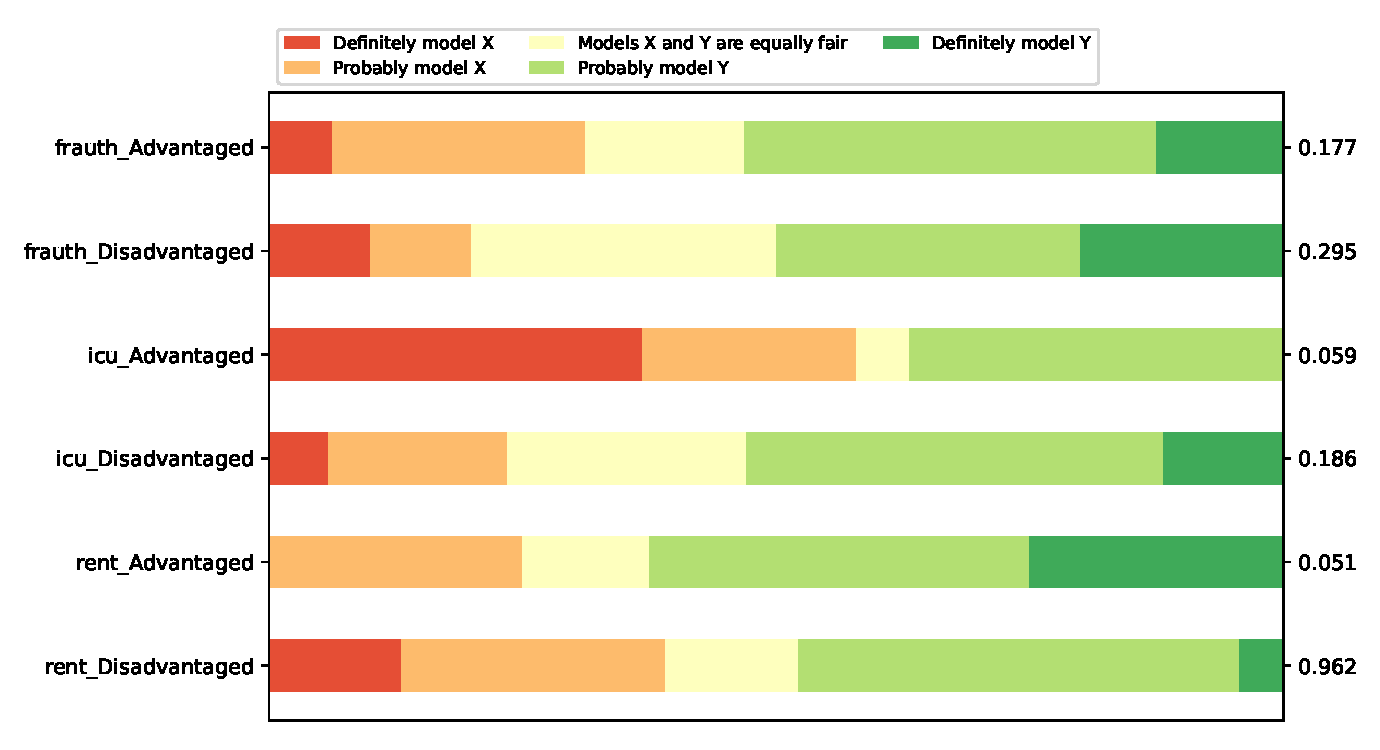
\includegraphics[width=0.8\textwidth]{figures/Q10.14/09202021_10082021_10312021_11092021/Q10.14_scenario_PGM.pdf}
    \caption{Grouped by scenario \& PGM}
    \label{fig:my_label}
\end{figure}
